\section{\'Etude des performances}

L'étude des performances se concentre sur deux aspects à optimiser de manière générale en programmation parallèle : les communications entre processus et la répartition des calculs dans ces processus. Le premier aspect est abordé via l'influence sur les performances du calcul de la localisation des processus dans les différents n\oe uds de PlaFRIM. Le second est quand à lui étudié via le tracé des performances pour un nombre de processus croissant, faisant donc aparaître -- ou non -- la scalabilité du programme.

\subsection{Influence de la répartition des processus}

Sur la machine de test PlaFRIM, les processus peuvent être répartis sur plusieurs n\oe uds différents, nécessitant a priori des communications plus longues qu'entre les processus d'un même n\oe ud. Un \emph{benchmark} déterminant les temps d'exécutions de trois configurations de n\oe uds différentes en fonction de la taille du problème (taille des matrices) a donc été réalisé. Ces trois configurations contiennent toutes le même nombre de processus -- quatre --, répartis différemment sur les n\oe uds :
\begin{itemize}
\item 1 n\oe ud, 4 c\oe urs par n\oe ud ;
\item 2 n\oe uds, 2 c\oe urs par n\oe ud ;
\item 4 n\oe uds, 1 c\oe ur par n\oe ud.
\end{itemize}
Les temps d'exécutions des trois configurations sont identiques quelque soit la taille du problème, en effet les courbes de la figure \ref{graph:sizes} sont toutes confondues. Nous pouvons donc penser que les communications entre n\oe uds sont dans notre cas -- i. e. pour le nombre de communications que requiert la multiplication de Fox pour des matrices jusqu'à la taille $3000$ et pour $4$ processus -- aussi performantes que les communications dans un même n\oe ud.

\begin{figure}
\begin{center}
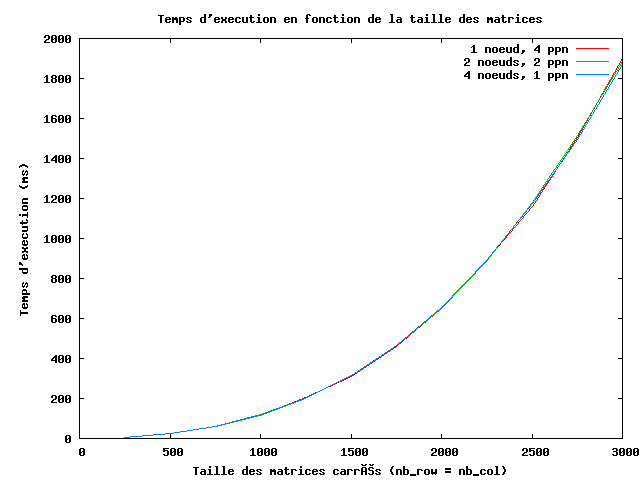
\includegraphics[scale=0.45]{graph_sizes.png}
\caption{Temps d'exécution en fonction de la taille du problème, pour trois répartitions différentes de processus.}
\label{graph:sizes}
\end{center}
\end{figure}

\subsection{Scalabilité du programme}

La scalabilité du programme correspond à l'accélération que peut fournir l'utilisation d'un nombre de processus supérieur à $1$ pour effectuer le calcul étudié. \'Etant donné que la multiplication de Fox est ici effectuée sur des matrices carrés, nous utilisons toujours le nombre de processus maximum étant un carré d'entier. Par exemple si $10$ processus sont fournis pour le calcul, seuls $9$ seront utilisés.

Afin de vérifier les performances en matière de scalabilité, le \emph{benchmark} réalisé est le tracé du temps d'exéction pour une taille du problème fixée, en fonction du nombre de processus fournis. Sur les graphiques, des palliers aparaissent entre les différents carrés d'entiers -- pour le nombre de processus --, ce qui est en adéquation avec la remarque du paragraphe ci-dessus sur le nombre de processus réellement utilisés. 

\begin{figure}
\begin{center}
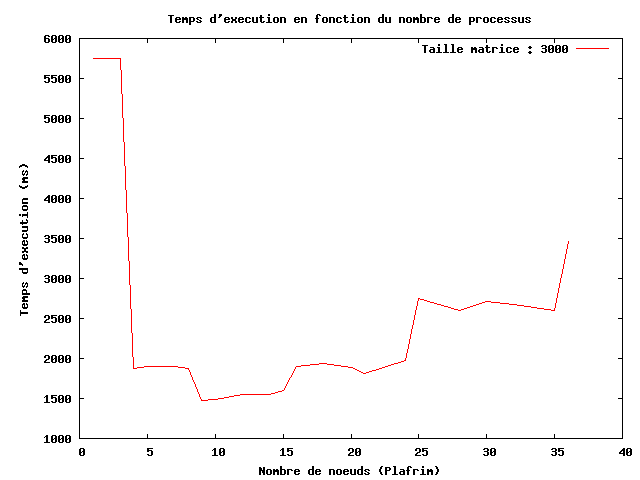
\includegraphics[scale=0.45]{graph_procs.png}
\caption{Temps d'exécution en fonction du nombre de processus. Taille du problème : 3000.}
\label{graph:procs}
\end{center}
\end{figure}

Cependant, comme nous pouvons le constater sur la figure \ref{graph:procs}, le temps d'exécution ne fait pas que diminuer lorsque le nombre de processus augmente -- au-delà d'un nombre de processus de $16$ -- mais au contraire il augmente de nouveau, en restant toutefois inférieur au temps séquentiel. Nous ne nous expliquons pas ce phénomène, mis à part le fait que ces tests ont été réalisés lorsque PlaFRIM n'était pas encore entièrement rétablie que nous n'avons donc pas la garantie que le bon nombre de processus aient été lancés au-delà de $4$ n\oe uds utilisés.

Notons que nous pouvons déduire de la figure \ref{graph:procs} des \emph{speedups} de l'ordre de $3$ pour l'utilisation de $4$ processus, et de $4$ pour l'utilisation de $9$ processus.

Par ailleurs nous pouvons remarquer que pour des tailles du problème relativement faible -- $500$ éléments par ligne/colonne -- le coût des communications est très élevés et dépasse largement le temps de calcul ce qui provoque des temps d'exécutions en parallèle bien supérieurs que le temps séquentiel, comme il est visible sur la figure \ref{graph:proc}.

\begin{figure}
\begin{center}
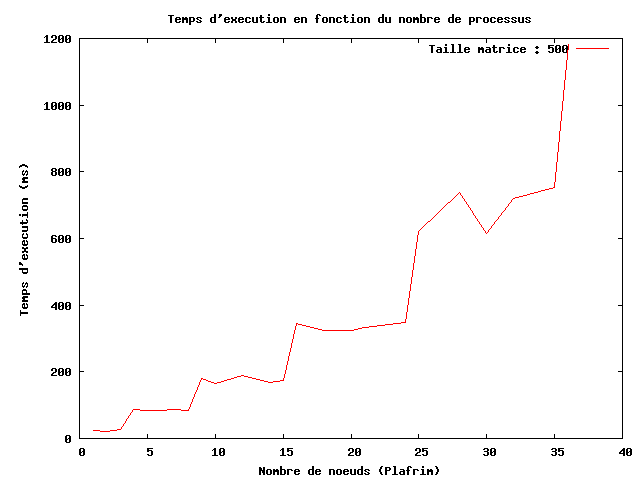
\includegraphics[scale=0.45]{graph_procs_500.png}
\caption{Temps d'exécution en fonction du nombre de processus. Taille du problème : 500.}
\label{graph:proc}
\end{center}
\end{figure}

